% Content of Worksheet 03, shared by the problem sheet and the solution sheet.
% Solutions are wrapped in the `solution` environment and appear only when the
% driver defines \ipsshowsolutions.

\ipsmaketitle

This worksheet is ungraded practice, with the same shape and level as the final exam.
Plan up to 2 hours for a serious pass.
Work each problem through on paper before you open the solutions, and show your algebra:
the exam asks for the steps, not only the number.
Some parts state an intermediate result (``show that\,\ldots''); use it to check your work, and to continue if a step resists.
Carry at least four significant figures through the intermediate steps (the worked solutions print five) and round only at the end.
All parts are analytical; no computer is needed.

\begin{given}[Constants and data]
$\kB = 1.381 \times 10^{-23}\ \mathrm{J\,K^{-1}}$ \quad
$m_u = 1.661 \times 10^{-27}\ \mathrm{kg}$ \quad
$\sigma = 5.670 \times 10^{-8}\ \mathrm{W\,m^{-2}\,K^{-4}}$ \quad
$S_\oplus = 1361\ \mathrm{W\,m^{-2}}$ (solar constant at 1 AU) \quad
$\Mearth = 5.972 \times 10^{24}\ \mathrm{kg}$

\vskip4pt
Earth: $P_0 = 1.013 \times 10^{5}$ Pa, $\Rearth = 6371$ km, $T_{\mathrm{eff}} = 255$ K, surface $288$ K, $\Omega = 7.29 \times 10^{-5}\ \mathrm{rad\,s^{-1}}$, $\Gamma_d = 9.8\ \mathrm{K\,km^{-1}}$

\vskip4pt
Water: $L_v = 2.50 \times 10^{6}\ \mathrm{J\,kg^{-1}}$, $R_v = 462\ \mathrm{J\,kg^{-1}\,K^{-1}}$ ($L_v/R_v = 5400$ K), triple point $(273\ \mathrm{K},\ 611\ \mathrm{Pa})$

\vskip6pt
\begin{tabular}{@{}lcccc@{}}
\toprule
Body & $T$ (K) & $\mu$ & $g$ (m\,s$^{-2}$) & Bond albedo $A$ \\
\midrule
Venus (0.72 AU) & 737 (surface) & 43.4 & 8.87 & 0.77 \\
Earth (1 AU)    & 288 (surface) & 28.97 & 9.81 & 0.30 \\
Titan           & 94 (surface)  & 28.6 & 1.35 & --- \\
\bottomrule
\end{tabular}

\vskip4pt
{\footnotesize Atmospheric data as in the Lecture 5 notes; $\mu$ is dimensionless, in units of $m_u$. The young Sun had $L/\Lsun = 0.71$ (Lecture 6 notes).}
\end{given}


% ════════════════════════════════════════════════════════════
\problem{How thick is an atmosphere?}

The scale height sets the thickness of every atmosphere in the solar system,
and hydrostatic balance connects the surface pressure to the mass sitting overhead.

\parti Compute the scale height $H = \kB T / (\mu\,m_u\,g)$ for Earth and for Titan.

\begin{solution}
For Earth, with $T = 288$ K, $\mu = 28.97$, $g = 9.81\ \mathrm{m\,s^{-2}}$:
\begin{align*}
H_\oplus &= \frac{\kB T}{\mu\,m_u\,g}
= \frac{1.381 \times 10^{-23} \times 288}{28.97 \times 1.661 \times 10^{-27} \times 9.81}
= \frac{3.9773 \times 10^{-21}}{4.7205 \times 10^{-25}} = 8425.6\ \mathrm{m} \approx 8.426\ \mathrm{km}.
\end{align*}
For Titan, with $T = 94$ K, $\mu = 28.6$, $g = 1.35\ \mathrm{m\,s^{-2}}$:
\begin{align*}
H_{\mathrm{Titan}} &= \frac{1.381 \times 10^{-23} \times 94}{28.6 \times 1.661 \times 10^{-27} \times 1.35}
= \frac{1.2981 \times 10^{-21}}{6.4131 \times 10^{-26}} = 20241\ \mathrm{m} \approx 20.24\ \mathrm{km},
\end{align*}
matching the table in the Lecture 5 notes (8.4 and 20 km).
\end{solution}

\parti Titan is far colder than Earth, and its nitrogen atmosphere has nearly the same $\mu$ as air.
Explain, from the structure of the scale-height formula, why Titan's atmosphere is nonetheless more than twice as extended as Earth's.

\begin{solution}
The scale height compares thermal energy $\kB T$ against the gravitational confinement $\mu m_u g$.
Titan's temperature is lower by a factor of about 3 ($94$ vs $288$ K), which by itself would compress the atmosphere.
But Titan's surface gravity is weaker by a factor of about 7 ($1.35$ vs $9.81\ \mathrm{m\,s^{-2}}$), and $H \propto T/g$ with $\mu$ essentially equal for the two nitrogen atmospheres.
The gravity ratio wins: $(288/94) \approx 3.1$ against $(9.81/1.35) \approx 7.3$, so $H_{\mathrm{Titan}}/H_\oplus \approx 7.3/3.1 \approx 2.4$.
Weak confinement, not warmth, is what puffs up Titan's atmosphere.
\end{solution}

\parti Integrate hydrostatic balance $\dd P = -\rho g\,\dd z$ over the whole column to show that
the surface pressure equals the weight per unit area of the overlying gas, $P_0 = m_{\mathrm{col}}\,g$,
where $m_{\mathrm{col}}$ is the column mass per unit area.
Evaluate $m_{\mathrm{col}}$ for Earth,
and from it the total mass of Earth's atmosphere.

\begin{solution}
Integrating from the surface to the top of the atmosphere, where $P \to 0$:
$$
P_0 - 0 = \int_0^{\infty} \rho g\,\dd z = g \int_0^{\infty} \rho\,\dd z = g\,m_{\mathrm{col}},
$$
with $g$ taken constant over the thin atmospheric shell. Therefore
$$
m_{\mathrm{col}} = \frac{P_0}{g} = \frac{1.013 \times 10^{5}}{9.81} = 1.0326 \times 10^{4}\ \mathrm{kg\,m^{-2}},
$$
about ten tonnes of air on every square metre.
The total atmospheric mass is the column mass times the surface area:
$$
M_{\mathrm{atm}} = 4\pi \Rearth^2\,m_{\mathrm{col}} = 4\pi\,(6.371 \times 10^{6})^2 \times 1.033 \times 10^{4} = 5.269 \times 10^{18}\ \mathrm{kg},
$$
about one millionth of Earth's mass.
\end{solution}


% ════════════════════════════════════════════════════════════
\problem{Sunlight in, infrared out}

Radiative equilibrium sets the temperature every atmosphere starts from;
the greenhouse effect explains why surfaces are warmer than that.

\parti Compute the solar flux at Venus's orbit,
then the equilibrium temperature of Venus,
$$
T_{\mathrm{eq}} = \left[\frac{(1 - A)\,S}{4\sigma}\right]^{1/4},
$$
and compare it with the value in the Lecture 5 notes.

\begin{solution}
The flux falls off with the inverse square of distance:
$$
S_{\mathrm{Venus}} = \frac{S_\oplus}{(0.72)^2} = \frac{1361}{0.5184} = 2625.4\ \mathrm{W\,m^{-2}}.
$$
With $A = 0.77$:
$$
T_{\mathrm{eq}} = \left[\frac{0.23 \times 2625.4}{4 \times 5.670 \times 10^{-8}}\right]^{1/4}
= \left[2.6624 \times 10^{9}\ \mathrm{K^4}\right]^{1/4} = 227.2\ \mathrm{K},
$$
matching the notes' 227 K. Venus's brilliant clouds reflect so much sunlight that its equilibrium
temperature is lower than Earth's 255 K, despite Venus being closer to the Sun.
\end{solution}

\parti Venus's measured surface temperature is 737 K, more than 500 K above the value you just computed.
Explain the mechanism that maintains this difference. Your answer must name the quantity that the
atmosphere blocks, and why blocking it raises the surface temperature.

\begin{solution}
The 92-bar $\mathrm{CO_2}$ atmosphere is nearly transparent to incoming sunlight but nearly opaque to
the outgoing thermal infrared radiated by the surface.
The surface can only shed energy through an atmosphere that absorbs and re-emits infrared many times over,
part of it back downward.
To push the same absorbed solar power out through this blanket, the surface must radiate far more strongly,
which by the Stefan-Boltzmann law means it must be far hotter.
The equilibrium temperature still describes what the planet radiates to space, but that radiation now
leaves from cold, high atmospheric layers rather than from the ground.
\end{solution}

\parti A fellow student writes: ``back-radiation from the atmosphere is a second energy source,
so the surface receives more energy than the Sun provides, and that violates energy conservation.''
Judge this claim and correct what is wrong with it.

\begin{solution}
The observation is right and the conclusion is wrong.
The surface does receive more radiative energy than the direct sunshine alone (on Earth, the downward
infrared from the atmosphere is even larger than the absorbed solar flux), but the atmosphere is not a
source: it only returns part of the energy the surface itself radiated upward.
Every joule still originates from the Sun, and at the top of the atmosphere absorbed sunlight and
outgoing infrared balance exactly.
Energy is conserved at every level; the greenhouse effect only slows the escape of energy and raises the
temperature the surface needs to pass its share outward.
\end{solution}


% ════════════════════════════════════════════════════════════
\problem{From vapour to cloud base}

The Clausius-Clapeyron equation from the blackboard derivation of Lecture 6 predicts where clouds
form. The figure below reproduces the saturation curves from the notes; part (b) reads it.

\begin{center}
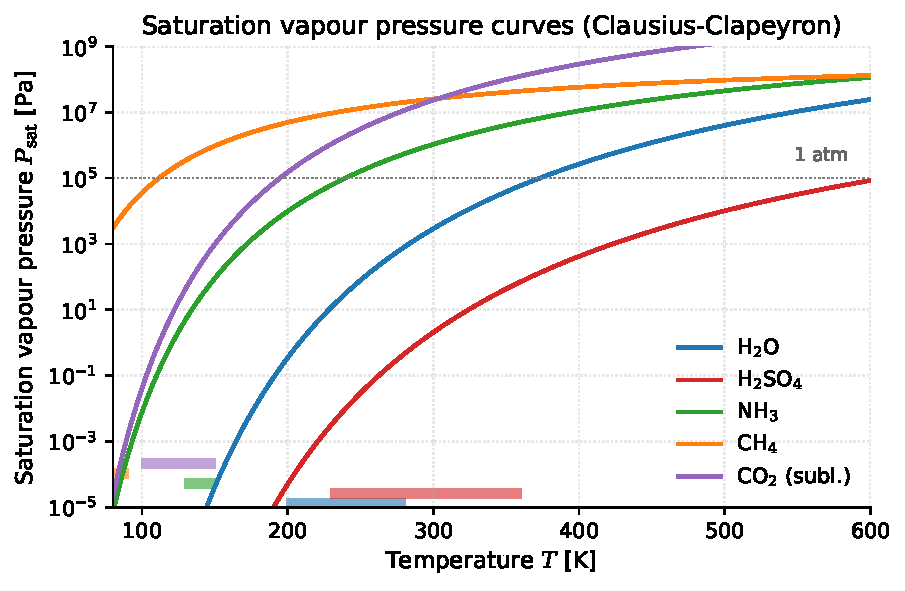
\includegraphics[width=0.62\linewidth]{figures/psat_curves}
\end{center}

\parti A parcel at the surface has $T = 293$ K and relative humidity 50\%.
Use the integrated Clausius-Clapeyron equation with the triple point of water as the reference state
to compute its vapour pressure (show that $P_{\mathrm{sat}}(293\ \mathrm{K}) \approx 2357$ Pa and
$P_{\mathrm{vap}} \approx 1179$ Pa), invert the Clausius-Clapeyron equation for the dew point
(show that $T_d \approx 282.4$ K), and from the dry adiabatic cooling rate find the altitude
of the cloud base. Take the vapour pressure as constant during ascent.

\begin{solution}
First the saturation pressure at the surface temperature:
$$
P_{\mathrm{sat}}(293) = 611\,\exp\!\left[-5400\left(\frac{1}{293} - \frac{1}{273}\right)\right]
= 611\,\exp(1.3502) = 2357\ \mathrm{Pa},
$$
so at 50\% relative humidity $P_{\mathrm{vap}} = 0.5 \times 2357 = 1179$ Pa (checkpoints match).
The dew point is the temperature at which this vapour pressure saturates. Inverting the Clausius-Clapeyron equation:
$$
\frac{1}{T_d} = \frac{1}{273} - \frac{\ln(P_{\mathrm{vap}}/611)}{5400}
= 3.6630 \times 10^{-3} - \frac{\ln(1.9296)}{5400} = 3.5413 \times 10^{-3}\ \mathrm{K^{-1}},
$$
so $T_d = 282.4$ K, matching the checkpoint. Rising air cools at $\Gamma_d = 9.8\ \mathrm{K\,km^{-1}}$
while its vapour pressure stays nearly constant, so condensation begins where the parcel temperature
meets the dew point:
$$
z_{\mathrm{LCL}} = \frac{T - T_d}{\Gamma_d} = \frac{293 - 282.4}{9.8} = 1.082\ \mathrm{km}.
$$
This is the lifting condensation level, and it sits exactly in the 1--2 km range the notes quote for
Earth's typical cloud base.
\end{solution}

\parti Read the saturation-curve figure: a body with a solid surface has regions at $90$ K where one
atmospheric gas is present at a partial pressure of about $10^4$ Pa ($0.1$ bar). Identify from the
figure which of the five species is at its saturation point under these conditions, and hence which
body in the solar system this is. Justify your reading in one or two sentences.

\begin{solution}
At 90 K, only the $\mathrm{CH_4}$ curve passes close to $10^4$ Pa: every other species has a saturation
pressure many orders of magnitude below that there ($\mathrm{H_2O}$, $\mathrm{CO_2}$, $\mathrm{NH_3}$,
$\mathrm{H_2SO_4}$ all lie far off the bottom of the plot at 90 K).
The gas is methane, at its saturation point.
The Lecture 6 table lists $\mathrm{CH_4}$ condensation on Titan, Uranus, and Neptune, but the ice giants
have no solid surface at these levels: the body with a surface is Titan.
The given-data table quotes 94 K for Titan's mean surface; the methane curve is so flat that both 90 and
94 K sit within a factor of two of saturation for a $\sim$0.1 bar methane partial pressure, which is
exactly why methane there cycles between vapour, rain, and lakes.
\end{solution}

\parti The Lecture 6 notes state that Venus's sulfuric-acid cloud base is sharply defined, while Titan's
methane clouds can form over a wide range of altitudes. Use the shape of the saturation curves in the
figure (steep for $\mathrm{H_2SO_4}$, flat for $\mathrm{CH_4}$) to explain both observations with the
same argument.

\begin{solution}
Condensation begins where the local vapour pressure crosses the saturation curve.
For $\mathrm{H_2SO_4}$, with its very large $L_v/R_v$, the saturation pressure changes by orders of
magnitude across a small temperature interval: descending droplets evaporate almost immediately below the
crossing, so the transition from clear air to cloud happens across a narrow altitude band and the cloud
base is sharp.
For $\mathrm{CH_4}$, the low $L_v/R_v$ makes the curve flat: methane vapour stays close to saturation
over a wide range of temperatures, so modest cooling anywhere in Titan's troposphere can push it over
the line, and clouds can appear across many kilometres of altitude.
One equation, two extremes of its exponential sensitivity.
\end{solution}


% ════════════════════════════════════════════════════════════
\problem{Winds on a rotating planet}

Rotation organises all large-scale flow.
Here you quantify it for the air above the Netherlands, then judge a claim.

\parti Compute the Coriolis parameter $f = 2\Omega\sin\phi$ for Groningen ($\phi = 53^\circ$N).

\begin{solution}
$$
f = 2 \times 7.29 \times 10^{-5} \times \sin 53^\circ = 1.458 \times 10^{-4} \times 0.79864
= 1.164 \times 10^{-4}\ \mathrm{s^{-1}}.
$$
The associated timescale $1/f \approx 2.4$ hours: any motion lasting longer
than a few hours feels the rotation.
\end{solution}

\parti A low-pressure system 2000 km across has winds of $15\ \mathrm{m\,s^{-1}}$.
Compute its Rossby number and state which force balance governs the flow.

\begin{solution}
$$
\mathrm{Ro} = \frac{U}{f L} = \frac{15}{1.164 \times 10^{-4} \times 2.0 \times 10^{6}} = 0.064.
$$
Since $\mathrm{Ro} \ll 1$, rotation dominates over inertia and the system is in geostrophic balance:
the pressure gradient force is balanced by the Coriolis force.
\end{solution}

\parti A fellow student writes: ``Venus rotates 243 times more slowly than Earth, so the Coriolis force
is weak, and its atmosphere must therefore break up into many more small circulation cells than Earth's.''
Judge this claim.

\begin{solution}
The premise is right and the conclusion is backwards.
Weak rotation means a weak Coriolis force, and it is the Coriolis deflection that breaks the
equator-to-pole overturning into separate cells: on Earth it halts the Hadley circulation near
30$^\circ$ and forces the three-cell structure.
With almost no deflection, Venus's overturning runs uninterrupted from equator to pole: one giant Hadley
cell per hemisphere, fewer cells, not more.
Many alternating cells are the signature of fast rotators such as Jupiter.
\end{solution}


% ════════════════════════════════════════════════════════════
\problem{Climate on the edge}

The energy-balance figure below reproduces the ice-albedo bistability diagram from the Lecture 6 notes;
you will need it in part (b).

\begin{center}
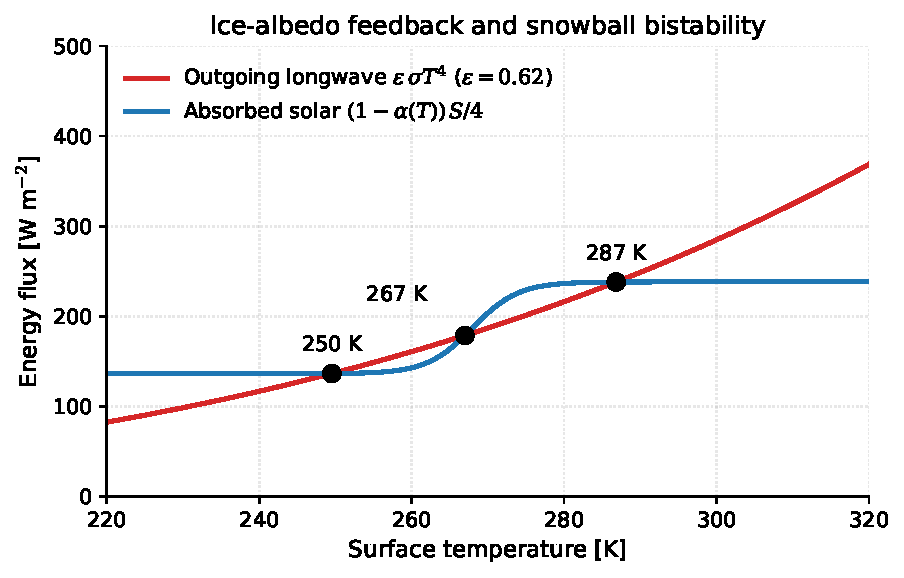
\includegraphics[width=0.58\linewidth]{figures/snowball_bistability_unlabeled}
\end{center}

\parti The young Sun shone at 71\% of its present luminosity.
Compute Earth's effective temperature at that time, taking today's albedo,
and state the paradox this number creates
when combined with the geological record.

\begin{solution}
Effective temperature scales as the fourth root of the absorbed flux, so
$$
T_{\mathrm{eff}} = 255 \times (0.71)^{1/4} = 255 \times 0.91794 = 234.1\ \mathrm{K}.
$$
With a greenhouse like today's ($+33$ K), the mean surface would sit near
$267$ K, well below freezing, and the oceans should have been ice.
Yet zircons, pillow basalts, and stromatolites record liquid water and life throughout the Archean.
A frozen prediction against a wet record: this is the faint young Sun paradox.
\end{solution}

\parti Read the bistability figure: identify which of the three intersections are stable and which is
unstable, and describe what happens to the climate if the planet sits at the middle intersection and is
nudged slightly toward warmer temperatures.

\begin{solution}
The outer two intersections are stable: at the 250 K crossing (snowball) and the 287 K crossing (warm
state), a small temperature excursion changes emission and absorption such that the planet is pushed
back toward the crossing.
The middle intersection at 267 K is unstable: it sits on the steep flank of the albedo transition.
Nudged warmer from 267 K, the planet melts some ice, absorbs more sunlight than it emits, and warms
further; the imbalance grows until the climate lands at the stable warm state at 287 K.
The same nudge cooler would run away into the snowball.
One incoming sunlight curve therefore supports two possible Earths, and history decides which one you
inhabit.
\end{solution}

\parti A large volcanic province doubles the volcanic $\mathrm{CO_2}$ outgassing rate for a few million
years. Using the carbonate-silicate cycle of Lecture 6, describe the chain of responses that returns
Earth's climate toward balance, and explain why this thermostat no longer works on Mars.

\begin{solution}
The extra $\mathrm{CO_2}$ strengthens the greenhouse and warms the surface.
A warmer, wetter climate speeds up silicate weathering, both through the Arrhenius-type temperature
dependence of the reactions and through increased rainfall.
Faster weathering draws $\mathrm{CO_2}$ out of the atmosphere and buries it as carbonate, so the
greenhouse weakens and the temperature relaxes back over a few hundred thousand years; the new steady
state is only modestly warmer, with weathering again matching the (elevated) outgassing.
On Mars the loop is broken at its source: volcanism largely ceased about 3 Gyr ago, so there is no
carbon resupply, and whatever $\mathrm{CO_2}$ weathering and escape removed was never returned.
A thermostat needs both a working sink and a working source; Mars kept neither.
\end{solution}

\parti A fellow student proposes: ``the faint young Sun paradox is solved because the early Earth had
more continental area than today, and rock absorbs more sunlight than water.''
Judge both halves of this claim against the Lecture 6 notes.

\begin{solution}
Both halves are wrong.
Continental crust grew over time: the early Earth had less land, not more, with most of the surface
under ocean.
And the albedo argument is inverted: ocean is darker than land, so a more water-covered Earth absorbs
more sunlight, not less.
The notes' albedo contribution to resolving the paradox rests exactly on this: a smaller continental
area (plus possibly fewer clouds) lowered the early Earth's albedo and helped the fainter Sun keep the
surface unfrozen, alongside the dominant contribution from a stronger $\mathrm{CO_2}$ and $\mathrm{CH_4}$
greenhouse.
\end{solution}
